% Generated with knitr; edit this Rnw source, not the output tex.


\section{Bootstrap calculation}
This chunk implements Algorithm~\ref{alg:bootstrap-mean}. The seed fixes the
random-number stream used for this demonstration. With only three
observations, the empirical distribution has very limited support; the
bootstrap interval below illustrates computation rather than reliable
coverage for a scientific application.

\begin{knitrout}
\definecolor{shadecolor}{rgb}{0.969, 0.969, 0.969}\color{fgcolor}\begin{kframe}
\begin{alltt}
\hlkwd{set.seed}\hldef{(}\hlnum{20260927}\hldef{)}
\hldef{B} \hlkwb{<-} \hlnum{2000L}
\hldef{alpha} \hlkwb{<-} \hlnum{0.05}
\hldef{boot_mean} \hlkwb{<-} \hlkwd{replicate}\hldef{(}
  \hldef{B,} \hlkwd{mean}\hldef{(}\hlkwd{sample}\hldef{(x,} \hlkwc{size} \hldef{= n,} \hlkwc{replace} \hldef{=} \hlnum{TRUE}\hldef{))}
\hldef{)}
\hlkwd{quantile}\hldef{(boot_mean,}
         \hlkwc{probs} \hldef{=} \hlkwd{c}\hldef{(alpha} \hlopt{/} \hlnum{2}\hldef{,} \hlnum{1} \hlopt{-} \hldef{alpha} \hlopt{/} \hlnum{2}\hldef{),} \hlkwc{names} \hldef{=} \hlnum{FALSE}\hldef{)}
\end{alltt}
\begin{verbatim}
## [1] 1 3
\end{verbatim}
\end{kframe}
\end{knitrout}

Report the seed, the number of resamples, the interval method, and software
versions in a reproducible
analysis. These bootstrap resamples are distinct from the independently
generated datasets used to estimate repeated-sampling coverage in a simulation
study.


\section{A figure generated by R}
Figure~\ref{fig:bootstrap-distribution} displays the empirical cumulative
distribution of the bootstrap means from Algorithm~\ref{alg:bootstrap-mean}.
Its steps reflect the limited support of the three-observation sample.
The vertical lines identify the observed mean and percentile endpoints.



\begin{knitrout}
\definecolor{shadecolor}{rgb}{0.969, 0.969, 0.969}\color{fgcolor}\begin{kframe}
\begin{alltt}
\hldef{endpoints} \hlkwb{<-} \hlkwd{quantile}\hldef{(}
  \hldef{boot_mean,} \hlkwc{probs} \hldef{=} \hlkwd{c}\hldef{(alpha} \hlopt{/} \hlnum{2}\hldef{,} \hlnum{1} \hlopt{-} \hldef{alpha} \hlopt{/} \hlnum{2}\hldef{),} \hlkwc{names} \hldef{=} \hlnum{FALSE}
\hldef{)}
\hlkwd{plot}\hldef{(}\hlkwd{ecdf}\hldef{(boot_mean),}
     \hlkwc{main} \hldef{=} \hlsng{""}\hldef{,} \hlkwc{xlab} \hldef{=} \hlsng{"Bootstrap sample mean"}\hldef{,}
     \hlkwc{ylab} \hldef{=} \hlsng{"Empirical cumulative probability"}\hldef{,}
     \hlkwc{verticals} \hldef{=} \hlnum{TRUE}\hldef{,} \hlkwc{do.points} \hldef{=} \hlnum{FALSE}\hldef{,} \hlkwc{xlim} \hldef{=} \hlkwd{c}\hldef{(}\hlnum{0.8}\hldef{,} \hlnum{3.2}\hldef{))}
\hlkwd{abline}\hldef{(}\hlkwc{v} \hldef{= x_bar,} \hlkwc{lty} \hldef{=} \hlnum{3}\hldef{)}
\hlkwd{abline}\hldef{(}\hlkwc{v} \hldef{= endpoints,} \hlkwc{lty} \hldef{=} \hlnum{2}\hldef{,} \hlkwc{col} \hldef{=} \hlsng{"blue"}\hldef{)}
\hlkwd{legend}\hldef{(}\hlsng{"topleft"}\hldef{,} \hlkwd{c}\hldef{(}\hlsng{"Observed mean"}\hldef{,} \hlsng{"Percentile endpoints"}\hldef{),}
       \hlkwc{lty} \hldef{=} \hlkwd{c}\hldef{(}\hlnum{3}\hldef{,} \hlnum{2}\hldef{),} \hlkwc{col} \hldef{=} \hlkwd{c}\hldef{(}\hlsng{"black"}\hldef{,} \hlsng{"blue"}\hldef{),} \hlkwc{bty} \hldef{=} \hlsng{"n"}\hldef{)}
\end{alltt}
\end{kframe}
\end{knitrout}

\begin{figure}[tbp]
\begin{knitrout}
\definecolor{shadecolor}{rgb}{0.969, 0.969, 0.969}\color{fgcolor}

{\centering 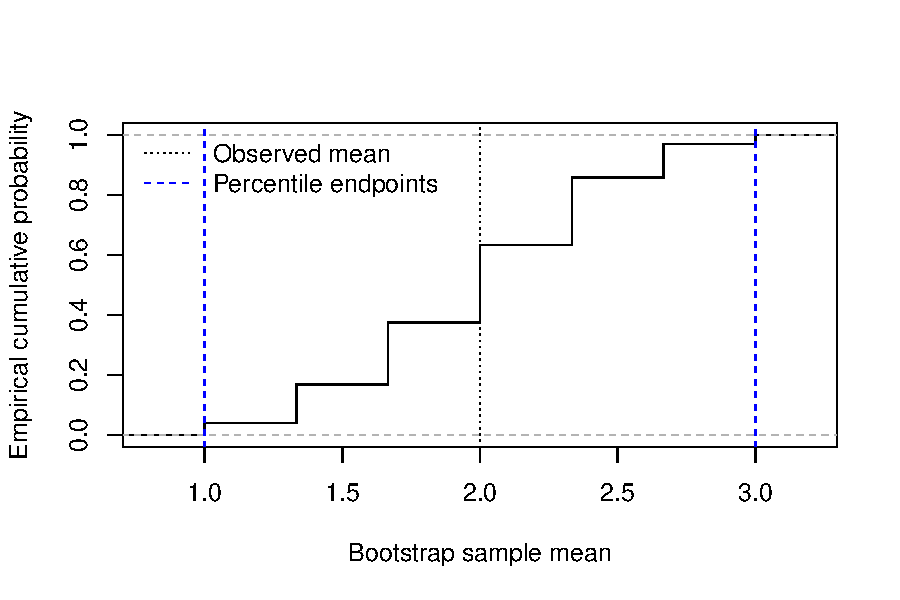
\includegraphics[width=\linewidth]{figures/bootstrap/bootstrap-distribution-1} 

}


\end{knitrout}

\caption[Empirical cumulative distribution of bootstrap means]{
Empirical cumulative distribution of 2,000 bootstrap means from the
observations 1, 2, and 3, using seed 20260927. The dotted line marks the
observed mean of 2; dashed lines mark the 95 percent percentile interval
endpoints of 1 and 3. This small-sample example illustrates computation,
not reliable coverage.}
\label{fig:bootstrap-distribution}
\end{figure}

Figure~\ref{fig:bootstrap-distribution} is generated by the R chunk.
Its caption and label are set explicitly with LaTeX commands in this Rnw
source. Use \verb|\ref| to refer to the figure number in the text.
The shorter caption appears in the list of figures; the full caption
explains the data and line styles.


\paragraph{Software versions.}
The following output records the versions used to generate this appendix.

\begin{knitrout}
\definecolor{shadecolor}{rgb}{0.969, 0.969, 0.969}\color{fgcolor}\begin{kframe}
\begin{verbatim}
## R version 4.6.1 (2026-06-24) 
## knitr 1.51
\end{verbatim}
\end{kframe}
\end{knitrout}
